\subsection{Preprocessing techniques}
In this section, we have implemented the preprocessing techniques we described above to different level of attacks, to be more specific the $\epsilon$ in FGSM attack. We then plot the accuracy of our net, with various values of parameters in different techniques.

\subsubsection{Bit-Depth Reduction}

\begin{figure}[h!]
	\centering
	\begin{subfigure}{.4\textwidth}
		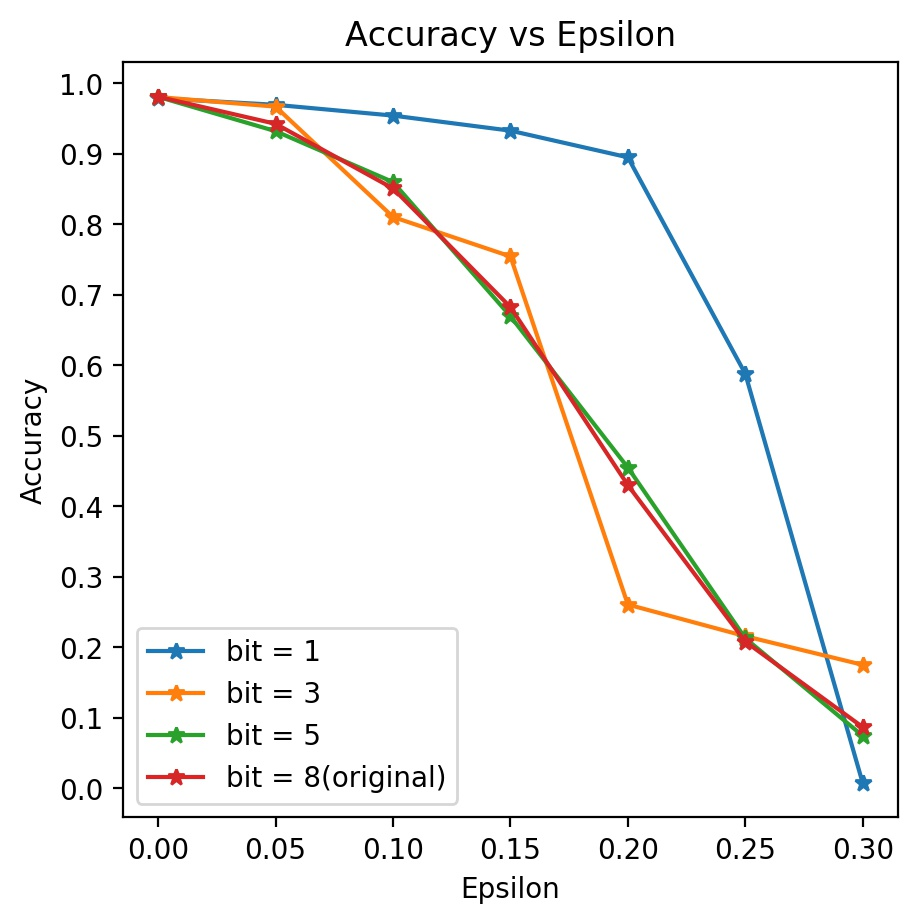
\includegraphics[width=\textwidth]{pretrained_Accuracy_vs_Epsilon_db.jpg}
		\caption{pretrained model}
		\label{fig: bit-depth reduction pre}
	\end{subfigure}
	\begin{subfigure}{.4\textwidth}
		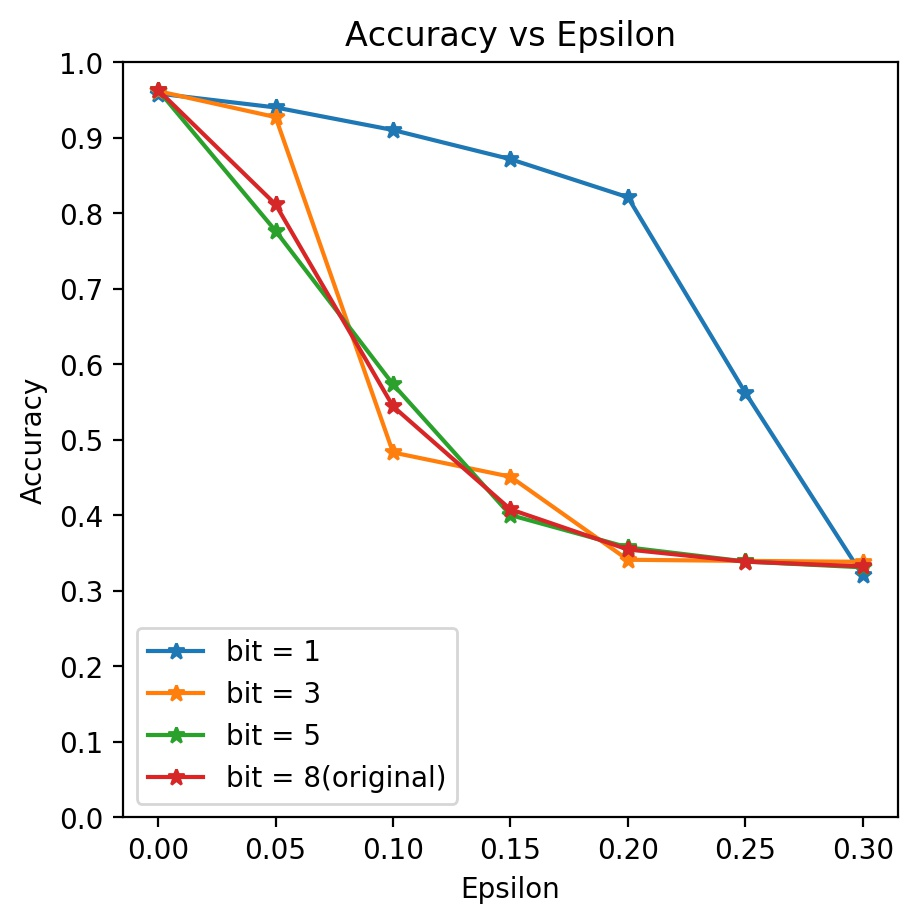
\includegraphics[width=\textwidth]{Accuracy_vs_Epsilon_db.jpg}
		\caption{Our model}
		\label{fig: bit-depth reduction us}
	\end{subfigure}
	\caption{Accuracy for different levels of noise we choose}
\end{figure}



\subsubsection{Total Variation}
\begin{figure}[h!]
	\centering
	\begin{subfigure}{.4\textwidth}
		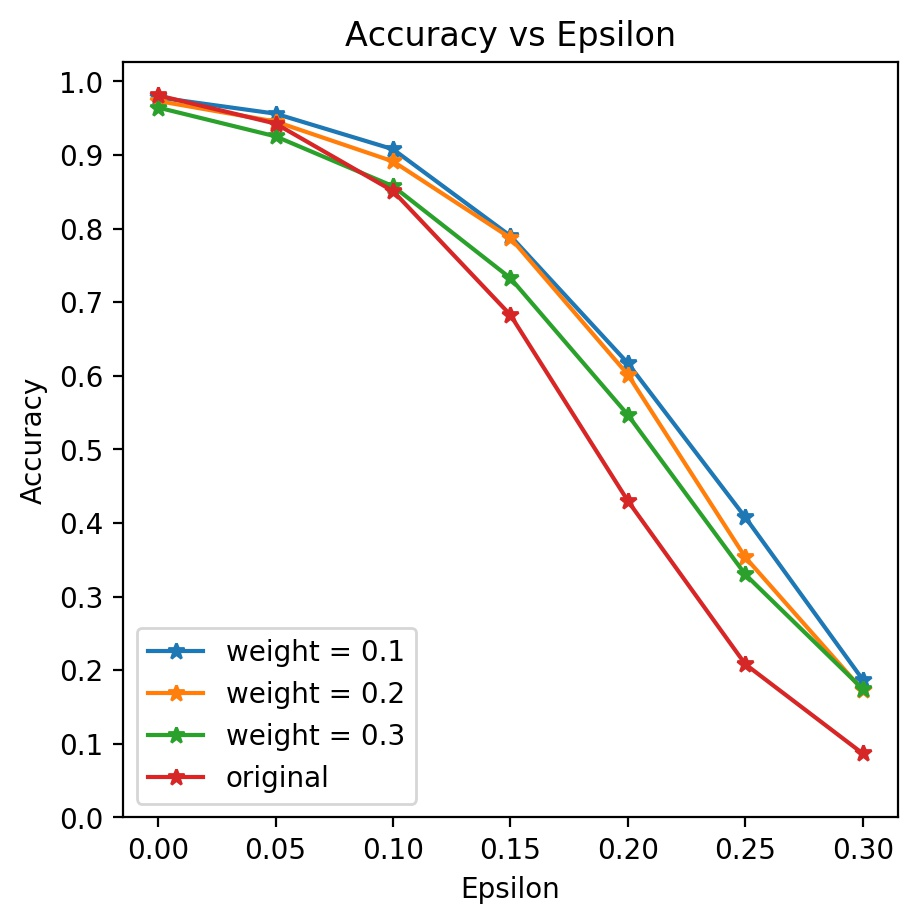
\includegraphics[width=\textwidth]{pretrained_Accuracy_vs_Epsilon_tv.jpg}
		\caption{pretrained model}
		\label{fig: tv pre}
	\end{subfigure}
	\begin{subfigure}{.4\textwidth}
		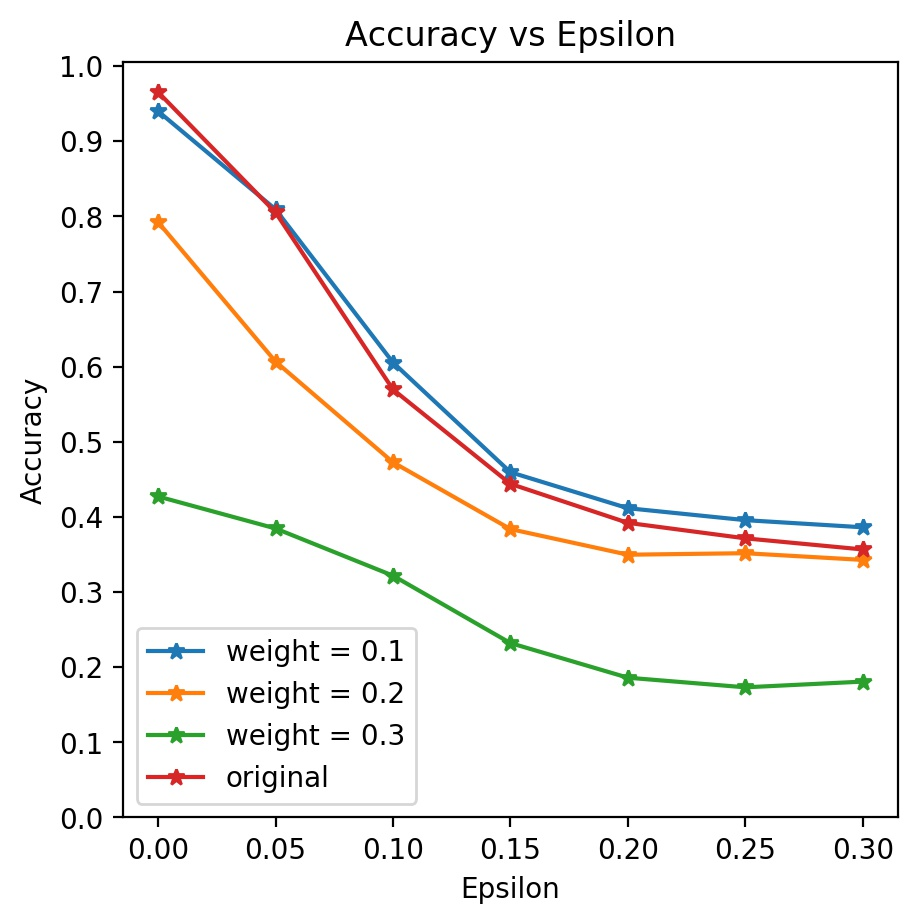
\includegraphics[width=\textwidth]{Accuracy_vs_Epsilon_tv.jpg}
		\caption{Our model}
		\label{fig: tv us}
	\end{subfigure}
	\caption{Accuracy for different levels of noise we choose}
\end{figure}